\documentclass[11pt]{article}
\usepackage[a4paper,margin=1in]{geometry}
\usepackage{amsmath,amssymb,amsthm,mathtools}
\usepackage{graphicx}
\usepackage[hidelinks]{hyperref}
\usepackage{xcolor}
\usepackage{microtype}

\newtheorem{theorem}{Theorem}
\newtheorem{lemma}{Lemma}
\newcommand{\R}{\mathbb R}
\newcommand{\N}{\mathbb N}
\newcommand{\Holder}[1]{C^{2,#1}}
\newcommand{\norm}[1]{\left\lVert #1\right\rVert}

\title{A flat elliptical function in \(\R^4\) that is not\\
a finite sum of regular squares}
\author{Candidate solution packet for arXiv:2107.12840}
\date{17 August 2026}

\begin{document}
\maketitle

\begin{abstract}
Korobenko and Sawyer call a function \emph{regular} when it belongs to
\(C^{2,\delta}\) for some \(\delta>0\), and construct elliptical flat smooth
functions not representable as finite sums of regular squares in dimensions
at least five.  We give such a function already on \(\R^4\).  The extra scale
coordinate in their construction is replaced by a sequence of disjoint hard
four-dimensional islands accumulating at the origin.  Their compactness
lower bound is diagonalized simultaneously over the number of squares and a
countable cofinal family of H\"older exponents.  No monotonicity property is
claimed.
\end{abstract}

\paragraph{Status and scope.}
This is a candidate counterexample.  It closes the unconstrained
dimension-four existence gap left by the source's \(n\geq5\) theorem.  It
does \emph{not} settle the separate question in source Remark~2.7 asking
whether specified weak monotonicity hypotheses force a positive result in
dimensions \(2,3,4\).

\section{Source input}

Set
\begin{equation}\label{eq:L}
 L(w,x,y,z)=w^4+x^2y^2+y^2z^2+z^2x^2-2wxyz.
\end{equation}
For \(0<\alpha<1\), let \(\mathcal C_{\nu,\alpha}(\tau)\) denote the
lower-bound function supplied by Korobenko--Sawyer, Lemma~5.2, for the modulus
\(\omega(t)=t^\alpha\).  The only source fact we use is
\begin{equation}\label{eq:source-hardness}
 \mathcal C_{\nu,\alpha}(\tau)\longrightarrow\infty
 \quad(\tau\downarrow0),
\end{equation}
and every identity on the unit ball
\begin{equation}\label{eq:source-identity}
 L+\tau=\sum_{j=1}^{\nu}h_j^2
\end{equation}
with \(h_j\in C^{2,\alpha}\) satisfies
\begin{equation}\label{eq:source-lower}
 \sum_{j=1}^{\nu}\norm{h_j}_{C^{2,\alpha}(B(0,1))}
 \geq \mathcal C_{\nu,\alpha}(\tau).
\end{equation}
This is a qualitative compactness assertion; no rate in \(\tau\) is needed.
Notice also that \(L\geq0\): AM--GM applied to the four nonnegative monomials
in \eqref{eq:L} gives a sum at least \(4|wxyz|\), which remains nonnegative
after subtracting \(2wxyz\).

\section{Proof intuition}

One hard copy of \(L\) multiplied by a flat factor does not suffice: after
normalizing the copy, derivatives of hypothetical square roots may acquire
an arbitrarily large inverse flat factor.  We instead put a separate copy
\(L+\tau_n\) in each of infinitely many tiny disjoint balls.  At the
\(n\)-th ball the normalization loss is a finite number \(R_n\), however
large.  We then choose \(\tau_n\) so small that the source lower bound exceeds
\(n^2R_n\) for every number of squares and every H\"older exponent among the
first \(n\) possibilities.  If one finite regular-square decomposition
existed, its rescaled norms would be at most \(CR_n\) on all late islands,
contradicting the chosen lower bound.

The island amplitudes are exponentially smaller than every power of their
radii.  Consequently all cutoff errors, including derivatives of every
order, disappear to infinite order at the sole accumulation point.

\section{The counterexample}

\begin{theorem}\label{thm:main}
There exists \(f\in C^\infty(\R^4;[0,\infty))\) such that
\begin{enumerate}
 \item \(f(0)=0\), \(f(x)>0\) for every \(x\neq0\), and every derivative of
 \(f\) vanishes at the origin;
 \item on no neighbourhood of the origin can \(f\) be written as
 \(f=\sum_{j=1}^{\nu}g_j^2\) for finitely many functions \(g_j\), each of
 which belongs to \(C^{2,\delta_j}\) for some \(\delta_j>0\).
\end{enumerate}
In particular, \(f\) is an elliptical flat smooth function on \(\R^4\) that
is not a finite sum of regular squares.
\end{theorem}

\begin{proof}
Write \(e_1=(1,0,0,0)\), and for \(n\geq1\) put
\begin{equation}\label{eq:scales}
 r_n=2^{-n-4},\qquad p_n=r_ne_1,\qquad
 \rho_n=\frac{r_n^2}{100},\qquad
 a_n=\exp(-\rho_n^{-2}).
\end{equation}
Choose \(\chi\in C_c^\infty(\R^4)\) with \(0\leq\chi\leq1\), equal to one
on \(B(0,1)\), and supported in \(B(0,2)\).  Set
\(\chi_n(x)=\chi((x-p_n)/\rho_n)\).  The closed supports are pairwise
disjoint: consecutive centers have distance \(r_n/2\), whereas
\[
 2\rho_n+2\rho_{n+1}
 =\frac{r_n^2}{40}<\frac{r_n}{2}.
\]
They also avoid the origin and accumulate only there.

For \(k,\nu\in\N\), abbreviate
\(\mathcal C_{\nu,k}=\mathcal C_{\nu,1/k}\), taking \(k\geq2\) when a
H\"older exponent below one is required.  Define the normalization loss
\begin{equation}\label{eq:Rn}
 R_n=1+\frac{\rho_nr_n+\rho_n^2}{\sqrt{a_n}}.
\end{equation}
By \eqref{eq:source-hardness}, for every \(n\) we may choose
\(0<\tau_n<1/n\) so small that
\begin{equation}\label{eq:diagonal}
 \mathcal C_{\nu,k}(\tau_n)\geq n^2R_n
 \quad\text{for all }1\leq\nu\leq n,\quad 2\leq k\leq n.
\end{equation}
Only finitely many conditions occur at each stage.

Let
\[
 b(x)=\begin{cases}\exp(-|x|^{-2}),&x\neq0,\\0,&x=0,\end{cases}
 \qquad
 F_n(x)=a_n\left[L\left(\frac{x-p_n}{\rho_n}\right)+\tau_n\right],
\]
and define
\begin{equation}\label{eq:f}
 f(x)=b(x)+\sum_{n=1}^\infty
 \chi_n(x)\bigl(F_n(x)-b(x)\bigr).
\end{equation}
Because the supports are disjoint, at most one summand is nonzero at each
point.  On a support, \(f=(1-\chi_n)b+\chi_nF_n\).  Both terms being positive
away from zero (and \(F_n>0\) because \(\tau_n>0\) and \(L\geq0\)), equation
\eqref{eq:f} is nonnegative and is strictly positive off the origin.

We next justify smoothness at the accumulation point.  On
\(B(p_n,2\rho_n)\) one has \(|x|\asymp r_n\).  For every derivative order
\(m\) and every \(N\), flatness of \(b\) gives
\[
 \sup_{B(p_n,2\rho_n)}|D^mb|=O_{m,N}(r_n^N).
\]
Leibniz' rule, \(D^q\chi_n=O_q(\rho_n^{-q})\), and the fixed degree of \(L\)
give, for every \(m\),
\begin{equation}\label{eq:flat-estimate}
 \sup_{B(p_n,2\rho_n)}
 \left|D^m\!\left[\chi_n(F_n-b)\right]\right|
 \leq C_m a_n\rho_n^{-m}+O_{m,N}(r_n^N\rho_n^{-m}).
\end{equation}
Since \(\rho_n=r_n^2/100\) and
\(a_n=\exp(-10^4r_n^{-4})\), the right side is \(o(r_n^A)\) for every
prescribed \(A\), after choosing \(N\) large in the second term.  Thus every
derivative of the correction in \eqref{eq:f} extends continuously to zero
with value zero.  Standard induction on the derivative order shows that
\(f\in C^\infty\) and all its derivatives vanish at zero.

It remains to exclude regular squares.  Suppose on some ball about zero that
\begin{equation}\label{eq:hyp-decomp}
 f=\sum_{j=1}^{\nu}g_j^2,
 \qquad g_j\in C^{2,\delta_j},\quad\delta_j>0.
\end{equation}
Let \(\delta=\min_j\delta_j\), and fix an integer \(k\geq2\) with
\(\alpha=1/k<\delta\).  On a smaller closed ball, all \(g_j\) have bounded
\(C^{2,\alpha}\) norms; denote a common bound by \(K\).

From \eqref{eq:hyp-decomp}, \(|g_j|\leq\sqrt f\).  Since \(f\) is flat,
\(\sqrt f=o(|x|^M)\) for every \(M\).  Hence every \(g_j\) is flat as a
function, and its \(C^2\) Taylor expansion implies
\begin{equation}\label{eq:jets}
 g_j(0)=0,\qquad Dg_j(0)=0.
\end{equation}

For all sufficiently large \(n\), the inner ball
\(B(p_n,\rho_n)\) lies in the decomposition domain and \(n\geq\max\{\nu,k\}\).
There \(\chi_n=1\), so after writing \(x=p_n+\rho_nW\) and setting
\begin{equation}\label{eq:G}
 G_{j,n}(W)=\frac{g_j(p_n+\rho_nW)}{\sqrt{a_n}},
\end{equation}
we obtain on \(B(0,1)\)
\begin{equation}\label{eq:scaled-id}
 L(W)+\tau_n=\sum_{j=1}^{\nu}G_{j,n}(W)^2.
\end{equation}

The function term in the \(C^{2,\alpha}\) norm is uniformly bounded because
\(|G_{j,n}|\leq\sqrt{L+\tau_n}\).  From \eqref{eq:jets}, the mean value
theorem, and the chain rule,
\begin{align*}
 \norm{DG_{j,n}}_\infty
 &\leq C K\frac{\rho_n(r_n+\rho_n)}{\sqrt{a_n}},\\
 \norm{D^2G_{j,n}}_\infty
 &\leq K\frac{\rho_n^2}{\sqrt{a_n}},\\
 [D^2G_{j,n}]_{\alpha}
 &\leq K\frac{\rho_n^{2+\alpha}}{\sqrt{a_n}}
 \leq K\frac{\rho_n^2}{\sqrt{a_n}}.
\end{align*}
Consequently a constant \(C_0\), depending on the alleged decomposition but
not on \(n\), satisfies
\begin{equation}\label{eq:upper}
 \sum_{j=1}^{\nu}\norm{G_{j,n}}_{C^{2,\alpha}(B(0,1))}
 \leq C_0R_n.
\end{equation}
On the other hand, the source estimate \eqref{eq:source-lower}, the diagonal
choice \eqref{eq:diagonal}, and \eqref{eq:scaled-id} imply that the same sum
is at least \(n^2R_n\).  Hence \(n^2\leq C_0\) for every sufficiently large
\(n\), an impossibility.  This proves the theorem.
\end{proof}

\section{Why the fifth coordinate is unnecessary here}

The source uses a fifth variable continuously to encode the scale and also
engineers a prescribed modulus of monotonicity.  For the unconstrained
existence problem, a discrete sequence of four-dimensional spatial islands
does the same diagonal job.  The key logical order is: first fix the island
geometry and amplitude, hence the finite loss \(R_n\); only then choose the
floor \(\tau_n\) using the unbounded compactness modulus.  Reversing that
order would create a circular rate requirement.

This observation does not automatically preserve any chosen
\(\omega\)-monotonicity.  Indeed, the relation between the tiny core floor
\(a_n\tau_n\) and surrounding values would require quantitative control of
the source hardness function, while Lemma~5.2 supplies only divergence.  The
dimension-four monotonicity threshold therefore remains outside the claim.

\section{Source evidence}

Figure~\ref{fig:p5} records the source definitions, Theorem~2.5 with its
\(n\geq5\) hypothesis, and Remark~2.7.  Figure~\ref{fig:p32} records the
hardness lemma used above.

\begin{figure}[ht]
\centering
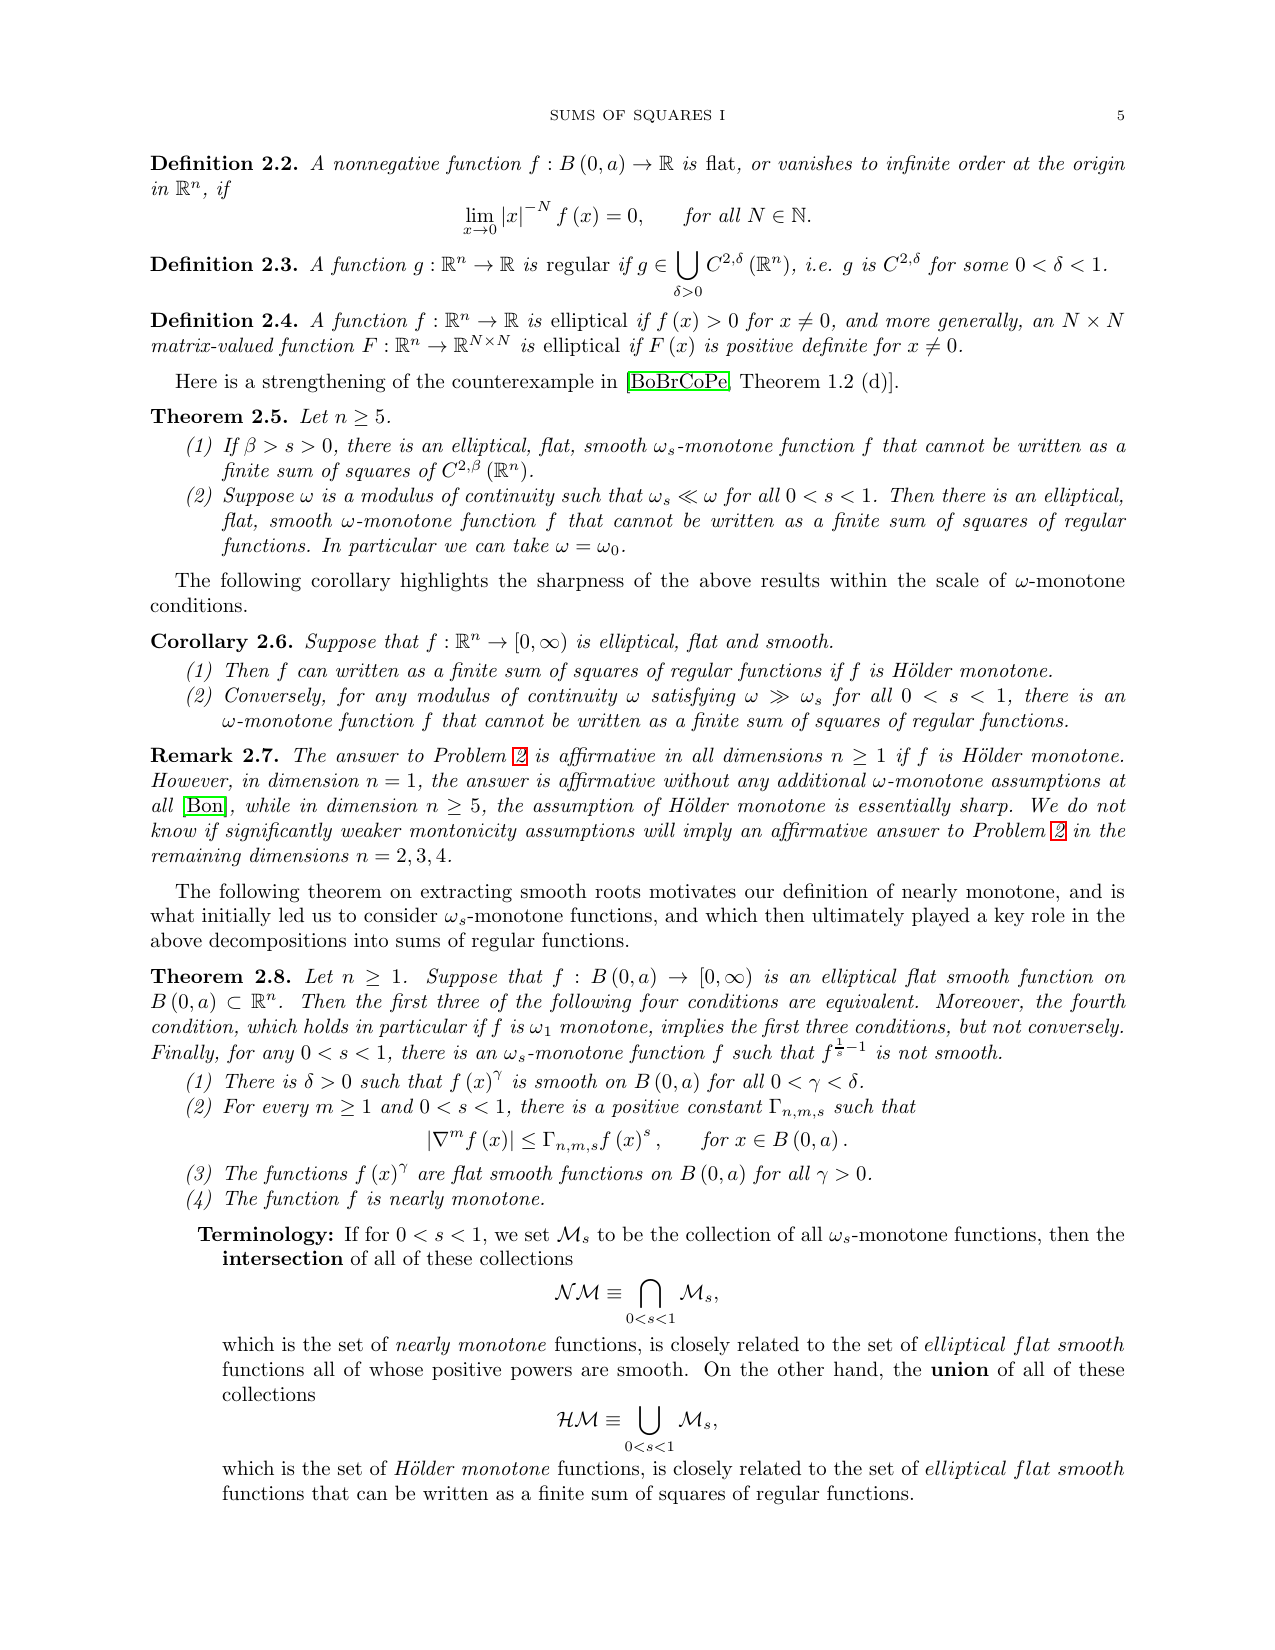
\includegraphics[width=\linewidth,trim=55bp 330bp 55bp 40bp,clip]{figures/source_page_5.png}
\caption{Korobenko--Sawyer, arXiv:2107.12840, PDF page 5 (cropped).}
\label{fig:p5}
\end{figure}

\begin{figure}[ht]
\centering
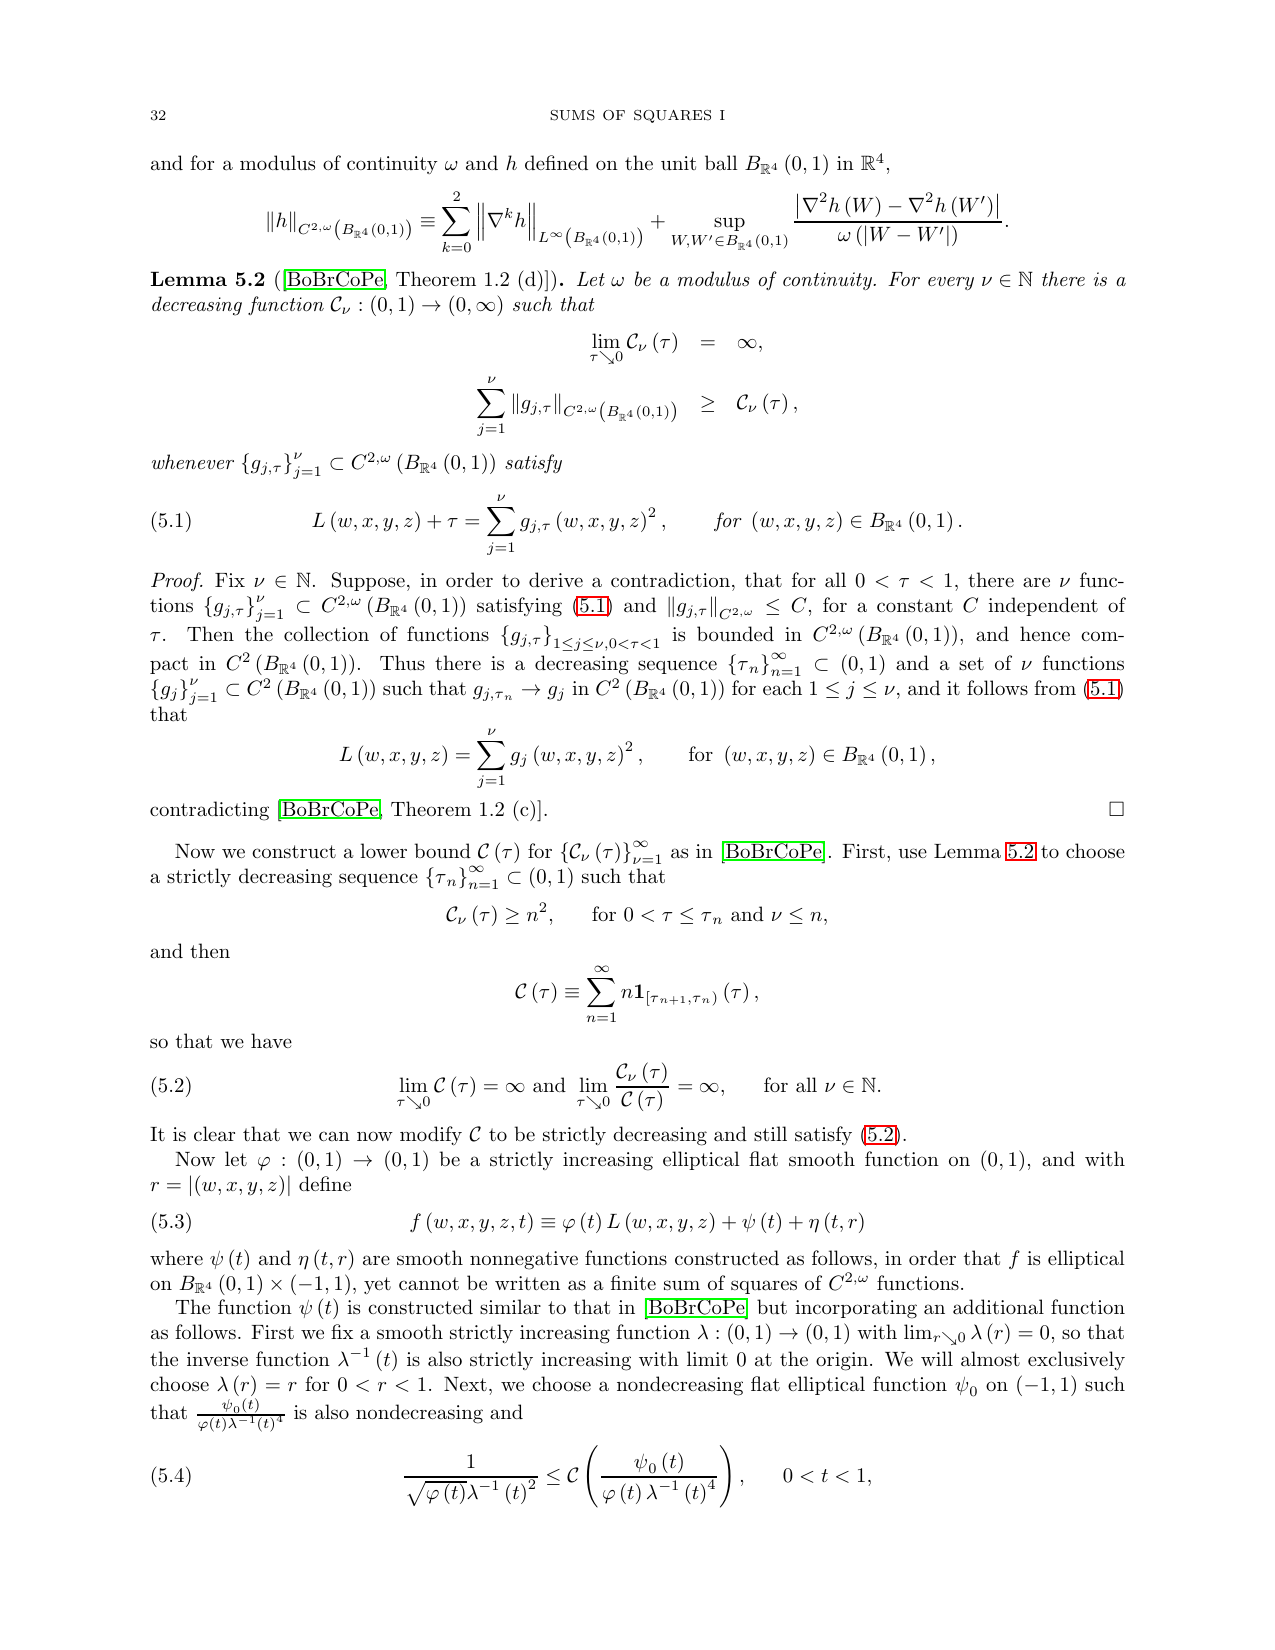
\includegraphics[width=\linewidth,trim=55bp 400bp 55bp 35bp,clip]{figures/source_page_32.png}
\caption{Korobenko--Sawyer, arXiv:2107.12840, PDF page 32 (cropped): the
\(C^{2,\omega}\) norm and Lemma~5.2.}
\label{fig:p32}
\end{figure}

\section*{References}

\noindent
[KS] S.~Korobenko and E.~T.~Sawyer,
\emph{Sum of squares I: scalar functions}, arXiv:2107.12840; Journal of
Functional Analysis 284 (2023), 109827.  In particular Definitions
2.2--2.4, Theorem~2.5, Remark~2.7, and Lemma~5.2.

\medskip
\noindent
[M] S.~MacDonald, \emph{Regularity preserving sum of squares
decompositions}, arXiv:2303.07998 (related polynomial obstructions; no claim
of overlap with the flat isolated-zero construction above).

\end{document}
